\chapter{引言}\label{chap:introduction}

\section{脑类器官}\label{sec:brain-organoid}
脑类器官是一种在体外人工培养的组织,其形态和功能类似于人类大脑的某些部分\cite{Kim2023}。
通过干细胞技术,科学家能够在实验室中培养出这些微型脑组织,用于研究大脑发育、疾病机制以及药物筛选等领域。
脑类器官的出现为神经科学研究提供了一个高度可控的实验平台,尤其是在研究复杂神经系统疾病时,其优势尤为明显。

\begin{figure}[!htbp]
    \centering
    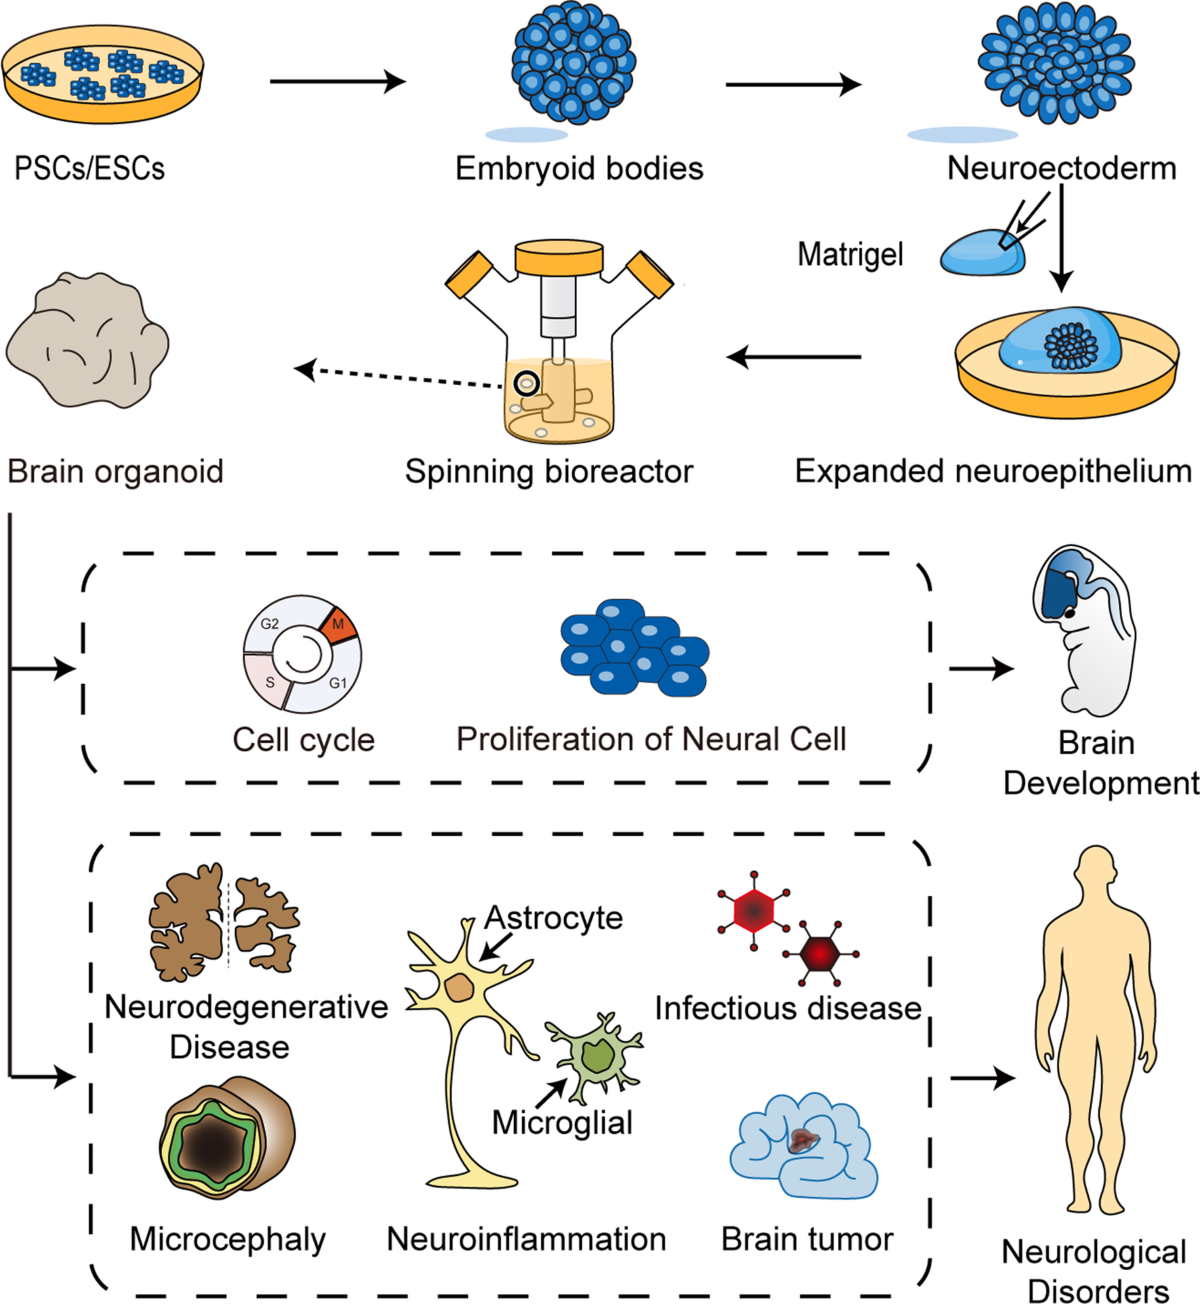
\includegraphics[width=0.50\textwidth]{Img/brain-organoid-flow.png}
    \bicaption{脑类器官的制备流程及用途\cite{facellitate_brain_organoids}}{The Preparation Process and Applications of Brain Organoids}
    \label{fig:brain-organoid-flow}
\end{figure}

\section{研究目的}\label{sec:research-purpose}
脑类器官的主要目的是在更加可控的环境中研究与大脑相关的疾病。
传统的动物模型虽然在一定程度上能够模拟人类大脑的功能,但由于物种差异,其研究结果往往难以直接应用于人类。
而脑类器官则能够更好地模拟人类大脑的发育和功能,为研究神经系统疾病提供了新的可能性。


\begin{figure}[!htbp]
    \centering
    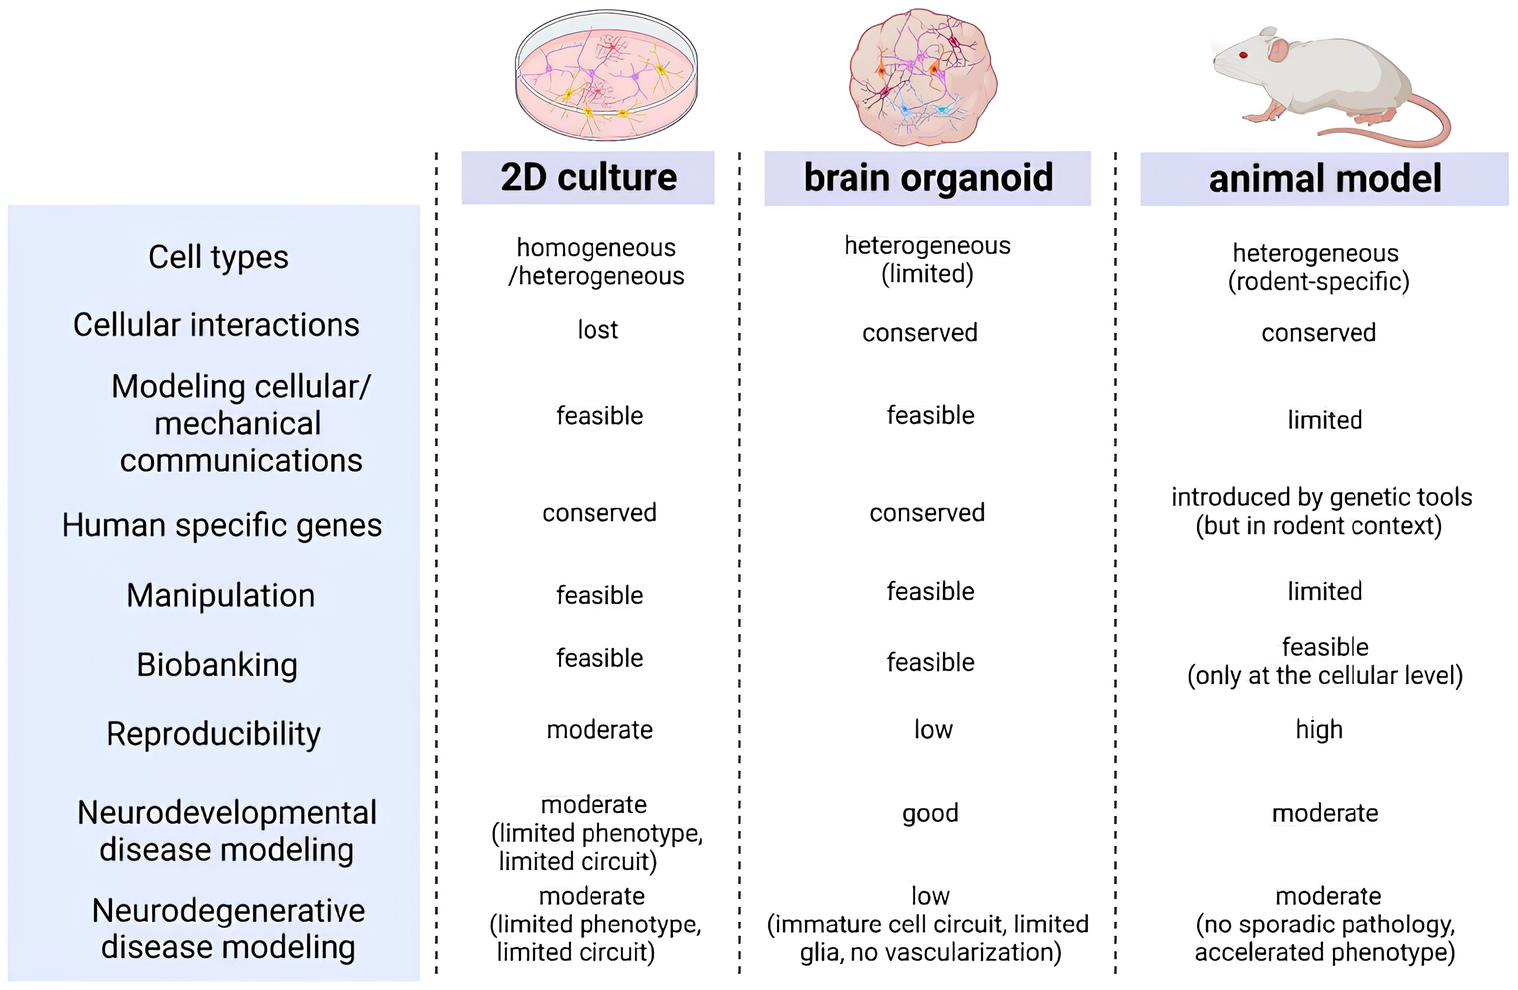
\includegraphics[width=0.75\textwidth]{Img/comparisons.png}
    \bicaption{脑类器官与其他模型的比较\cite{Kim2023}}{Comparisons of Brain Organoids with Other Models}
    \label{fig:comparisons}
\end{figure}

\section{面临的挑战}\label{sec:research-challenges}
尽管脑类器官在研究中展现出巨大的潜力,但其发展仍面临诸多挑战。
首先,从物理结构上来看,脑类器官的构建非常复杂。
大脑是一个高度复杂的器官,包含多个功能区域和复杂的血管结构,因此用现有技术培养一个真实比例的体外大脑的成本几乎是不可接受的;其次,从功能角度来看,脑类器官的功能发育也面临挑战。
即使能够构建出形态上相似的脑类器官,如何使其具备与真实大脑相似的神经元网络,以具备相似的功能,仍然是一个重要的研究方向。


\section{可能的解决方案}\label{sec:research-solutions}
针对上述挑战,研究者提出了两种可能的解决方案。
首先,从物理结构的角度,可以通过专注于重建特定的大脑区域来简化问题。
例如,选择重建海马体或前额叶皮层等特定区域,而不是试图重建整个大脑。
其次,从功能发育的角度,可以通过主动“训练”脑类器官,使其接受类似于真实大脑的完整刺激,从而促进其功能发育。
这种训练可以通过电刺激、化学刺激或光遗传学等手段实现。
